% Pandoc/Quarto template for den-paper extension
\documentclass[
  manuscript=article,
  layout=publish,
  year=2026,
  volume=6,
]{den}

% DOI

% Conference (for proceedings/poster)

% Dates
\published{7 July 2026}

% Editor and reviewers

% Strip abstract fields from bibliography entries (prevents LuaLaTeX parsing issues)

% Title
\title{A Behavioral Equilibrium Exchange Rate (BEER) Model for the
Indonesian Rupiah: Disentangling Fundamental, Domestic, and External
Drivers}

% Authors and affiliations
\author{Alfan Mansur \orcid{0000-0001-8695-0514}}
\affiliation{Dewan Ekonomi Nasional}
\email{alfanmansur@dewanekonomi.go.id}

% Keywords
\keywords{exchange rate; BEER; VECM; SVAR; Indonesian Rupiah}

% JEL classification codes
\jel{F31, C32, E58}

% Abbreviations

% Pandoc/Quarto compatibility macros
\providecommand{\tightlist}{%
  \setlength{\itemsep}{0pt}\setlength{\parskip}{0pt}}
\providecommand{\citeproc}[2]{#1}
\providecommand{\citeproctext}{}

% Support for graphics
\RequirePackage{graphicx}

% Support for ding symbols (checkmarks, etc.)
\RequirePackage{pifont}

% Support for table column width calculations (required by Quarto-generated tables)
\RequirePackage{calc}

% Pandoc image handling - required for newer Pandoc/Quarto versions
% Constrains images to text width to prevent overflow
\makeatletter
\providecommand{\pandocbounded}[1]{%
  \sbox0{#1}%
  \ifdim\wd0>\linewidth
    \resizebox{\linewidth}{!}{#1}%
  \else
    #1%
  \fi
}
\makeatother

% CSL references support
\newlength{\cslhangindent}
\setlength{\cslhangindent}{1.5em}
\newlength{\csllabelwidth}
\setlength{\csllabelwidth}{3em}
\makeatletter
\newcommand{\CSLNoBibLabel}{\renewcommand{\@biblabel}[1]{}}
\makeatother
\newenvironment{CSLReferences}[2]
 {\begin{list}{}%
  {\setlength{\leftmargin}{0pt}
   \setlength{\itemindent}{0pt}
   \setlength{\itemsep}{#2\baselineskip}
   \setlength{\parsep}{0pt}
   \setlength{\topsep}{0pt}
   \setlength{\partopsep}{0pt}
   \ifodd #1
     \setlength{\leftmargin}{\cslhangindent}
     \setlength{\itemindent}{-\cslhangindent}
   \fi}
  \CSLNoBibLabel}
 {\end{list}}

% Header includes
\makeatletter
\@ifpackageloaded{caption}{}{\usepackage{caption}}
\AtBeginDocument{%
\ifdefined\contentsname
  \renewcommand*\contentsname{Table of contents}
\else
  \newcommand\contentsname{Table of contents}
\fi
\ifdefined\listfigurename
  \renewcommand*\listfigurename{List of Figures}
\else
  \newcommand\listfigurename{List of Figures}
\fi
\ifdefined\listtablename
  \renewcommand*\listtablename{List of Tables}
\else
  \newcommand\listtablename{List of Tables}
\fi
\ifdefined\figurename
  \renewcommand*\figurename{Figure}
\else
  \newcommand\figurename{Figure}
\fi
\ifdefined\tablename
  \renewcommand*\tablename{Table}
\else
  \newcommand\tablename{Table}
\fi
}
\@ifpackageloaded{float}{}{\usepackage{float}}
\floatstyle{ruled}
\@ifundefined{c@chapter}{\newfloat{codelisting}{h}{lop}}{\newfloat{codelisting}{h}{lop}[chapter]}
\floatname{codelisting}{Listing}
\newcommand*\listoflistings{\listof{codelisting}{List of Listings}}
\makeatother
\makeatletter
\makeatother
\makeatletter
\@ifpackageloaded{caption}{}{\usepackage{caption}}
\@ifpackageloaded{subcaption}{}{\usepackage{subcaption}}
\makeatother

% Keep internal links clickable without PDF border underlines.
\hypersetup{pdfborder={0 0 0}}

% Source note environment for figure attributions (right-aligned, compact)
\newenvironment{source}{%
  \vspace{-1em}%
  \begin{flushright}\scriptsize\itshape
}{%
  \end{flushright}%
}
\newcommand{\sumber}[1]{%
  \vspace{-1em}%
  \begin{flushright}\scriptsize\itshape
  Sumber: #1
  \end{flushright}%
}

% Allow LaTeX more flexibility in line breaking to prevent overflow
% (needed for Indonesian/non-English text on narrow B5 paper)
\tolerance=1000
\emergencystretch=1.5em

\begin{document}

\begin{abstract}
This document provides the formal econometric and theoretical
documentation for a Behavioral Equilibrium Exchange Rate (BEER) model
applied to the Indonesian Rupiah (USD/IDR). Drawing on the foundational
framework of Clark and MacDonald (1998), the model evaluates whether the
currency's movements are driven by fundamental economic factors,
external sovereign risk sentiments, or domestic currency market noise.
Econometrically, the model is implemented via a Vector Error Correction
Model (VECM) to capture long-run cointegrating vectors, alongside a
Structural Vector Autoregression (SVAR) using a Cholesky identification
scheme to compute historical shock decompositions. The results provide a
systematic framework for exchange rate assessment and policy analysis in
the context of an emerging market economy.
\end{abstract}

\section{Introduction}\label{introduction}

Assessing whether an exchange rate is aligned with economic fundamentals
or driven by speculative and temporary shocks remains a core challenge
in empirical macroeconomics. Clark and MacDonald (1998) formalized the
Behavioral Equilibrium Exchange Rate (BEER) approach as an
econometrically driven alternative to the Fundamental Equilibrium
Exchange Rate (FEER) approach. While the FEER approach relies heavily on
subjective definitions of internal and external balance, the BEER
methodology utilizes cointegration techniques to establish direct
behavioral linkages between the actual real or nominal exchange rate and
its macroeconomic determinants.

The BEER approach is based on the idea that the actual real exchange
rate can be explained exhaustively in terms of a set of fundamental
variables, a set of variables that affect the exchange rate only in the
short run, and a random error (Clark and MacDonald 1998). Following
Clark and MacDonald (1998), the reduced-form expression for the real
exchange rate can be represented as:

\begin{equation}\phantomsection\label{eq-beer-general}{
q_t = \beta_1'Z_{1t} + \beta_2'Z_{2t} + \tau'T_t + \epsilon_t
}\end{equation}

where \(Z_1\) represents economic fundamentals expected to have
persistent effects over the long run, \(Z_2\) represents economic
fundamentals affecting the real exchange rate over the medium term,
\(T\) represents transitory factors affecting the real exchange rate in
the short run, and \(\epsilon_t\) is a random disturbance term.

The current equilibrium rate, \(q_t'\), is defined as the level of the
exchange rate given by the current values of the economic fundamentals
(Clark and MacDonald 1998):

\begin{equation}\phantomsection\label{eq-current-equilibrium}{
q_t' = \beta_1'Z_{1t} + \beta_2'Z_{2t}
}\end{equation}

Current misalignment, \(cm_t\), is defined as the difference between the
actual real exchange rate and the real exchange rate given by the
current values of all economic fundamentals:

\begin{equation}\phantomsection\label{eq-current-misalignment}{
cm_t = q_t - q_t' = \tau'T_t + \epsilon_t
}\end{equation}

Total misalignment, \(tm_t\), is defined as the difference between the
actual real rate and the real rate given by the sustainable or long-run
values of the economic fundamentals, \(\bar{Z}_{1t}\) and
\(\bar{Z}_{2t}\):

\begin{equation}\phantomsection\label{eq-total-misalignment}{
tm_t = q_t - \beta_1'\bar{Z}_{1t} - \beta_2'\bar{Z}_{2t}
}\end{equation}

Following Clark and MacDonald (1998), total misalignment can be
decomposed into current misalignment and the effect of departures of
current fundamentals from their long-run values:

\begin{equation}\phantomsection\label{eq-misalignment-decomposition}{
tm_t = \tau'T_t + \epsilon_t + [\beta_1'(Z_{1t} - \bar{Z}_{1t}) + \beta_2'(Z_{2t} - \bar{Z}_{2t})]
}\end{equation}

This framework is particularly well-suited for analyzing the Indonesian
Rupiah, a currency that has experienced significant volatility and is
influenced by both domestic macroeconomic conditions and external
financial market sentiment.

The primary objective of this model is to separate the structural
drivers of the currency into three distinct categories:

\begin{enumerate}
\def\labelenumi{\arabic{enumi}.}
\tightlist
\item
  Fundamentals: Core macroeconomic variables that determine long-run
  sustainability, including the terms of trade, net foreign assets,
  inflation differentials, and interest rate differentials.
\item
  External Risk Sentiment: Global and sovereign risk factors measured
  through the 5-year Credit Default Swap (CDS) spread.
\item
  Domestic Market Sentiment: Idiosyncratic shocks and short-term
  currency innovations captured via the exchange rate residual itself.
\end{enumerate}

\section{Theoretical Foundation}\label{theoretical-foundation}

\subsection{The Risk-Adjusted Interest Parity
Condition}\label{the-risk-adjusted-interest-parity-condition}

The starting point of our model follows Clark and MacDonald (1998),
beginning with the familiar risk-adjusted interest parity condition:

\begin{equation}\phantomsection\label{eq-risk-adjusted-interest-parity}{
E_t[\Delta s_{t+k}] = -(i_t - i_t^*) + \pi_t
}\end{equation}

where \(s_t\) is the foreign currency price of a unit of home currency,
\(i_t\) denotes a nominal interest rate, \(\pi_t = \lambda_t + \kappa\)
is the risk premium with a time-varying component \(\lambda_t\), and
\(E_t\) is the conditional expectations operator.

Following Clark and MacDonald (1998), this can be converted into a real
relationship by subtracting the expected inflation differential,
yielding:

\begin{equation}\phantomsection\label{eq-real-interest-parity}{
q_t = E_t[q_{t+k}] + (r_t - r_t^*) - \pi_t
}\end{equation}

where \(r_t = i_t - E_t(\Delta p_{t+k})\) is the ex ante real interest
rate. This equation describes the current equilibrium exchange rate as
being determined by three components: the expectation of the real
exchange rate in period \(t+k\), the real interest differential, and the
risk premium (Clark and MacDonald 1998).

\subsection{The Time-Varying Risk
Premium}\label{the-time-varying-risk-premium}

Following Clark and MacDonald (1998), the time-varying component of the
risk premium term is assumed to be a function of the relative supply of
domestic to foreign government debt:

\begin{equation}\phantomsection\label{eq-risk-premium-function}{
\lambda_t = g(gdebt_t / gdebt_t^*)
}\end{equation}

An increase in the relative supply of outstanding domestic debt relative
to foreign debt will increase the domestic risk premium, thereby
requiring a depreciation of the current equilibrium real exchange rate
(Clark and MacDonald 1998).

\subsection{Long-Run Equilibrium
Fundamentals}\label{long-run-equilibrium-fundamentals}

The long-run equilibrium exchange rate, \(\hat{q}_t\), is assumed to be
a function of three fundamental variables (Clark and MacDonald 1998):

\begin{equation}\phantomsection\label{eq-long-run-fundamentals}{
\hat{q}_t = f(tot_t, tnt_t, nfa_t)
}\end{equation}

where:

\begin{itemize}
\tightlist
\item
  \(tot\) is the terms of trade
\item
  \(tnt\) is the Balassa-Samuelson effect (relative price of nontraded
  to traded goods)
\item
  \(nfa\) is net foreign assets
\end{itemize}

The signs above the right-hand-side variables denote the partial
derivatives, indicating the expected direction of influence on the
equilibrium exchange rate (Clark and MacDonald 1998).

\section{Model Specification for the Indonesian
Rupiah}\label{model-specification-for-the-indonesian-rupiah}

\subsection{Variable Definitions and Data
Sources}\label{variable-definitions-and-data-sources}

The model is estimated using monthly time-series data from January 2010
to May 2026. The vector of endogenous variables is denoted as:

\begin{equation}\phantomsection\label{eq-variable-vector}{
Y_t = \begin{bmatrix} tot_t & nfa_t & infl\_diff_t & ir\_diff_t & cds_t & xr_t \end{bmatrix}'
}\end{equation}

Each variable is operationalized as follows:

\subsubsection{\texorpdfstring{Exchange Rate
(\(xr_t\))}{Exchange Rate (xr\_t)}}\label{exchange-rate-xr_t}

The natural logarithm of the nominal spot exchange rate (USD/IDR). An
increase represents a depreciation of the Rupiah. This variable is
measured as the monthly average of daily closing rates. \emph{Source}:
Bank Indonesia and Bloomberg.

\subsubsection{\texorpdfstring{Inflation Differential
(\(infl\_diff_t\))}{Inflation Differential (infl\textbackslash\_diff\_t)}}\label{inflation-differential-infl_diff_t}

The core inflation differential between Indonesia and the United States:

\begin{equation}\phantomsection\label{eq-inflation-differential}{
infl\_diff_t = Inflation_{IDN,t} - Inflation_{USA,t}
}\end{equation}

Core inflation is used to capture underlying price pressures, excluding
volatile food and energy components. \emph{Source}: Bank Indonesia and
U.S. Bureau of Labor Statistics.

\subsubsection{\texorpdfstring{Terms of Trade
(\(tot_t\))}{Terms of Trade (tot\_t)}}\label{terms-of-trade-tot_t}

The terms of trade index, reflecting the relative price of Indonesia's
exports to imports. This is defined as:

\begin{equation}\phantomsection\label{eq-terms-of-trade}{
tot_t = \frac{Export\ Price\ Index_t}{Import\ Price\ Index_t}
}\end{equation}

\emph{Source}: Bank Indonesia, World Bank, and IMF International
Financial Statistics.

\subsubsection{\texorpdfstring{Net Foreign Assets
(\(nfa_t\))}{Net Foreign Assets (nfa\_t)}}\label{net-foreign-assets-nfa_t}

The net external asset position of the economy, expressed as a ratio to
GDP. This variable captures the stock equilibrium condition in the
external sector. \emph{Source}: Bank Indonesia and IMF International
Investment Position statistics.

\subsubsection{\texorpdfstring{Interest Rate Differential
(\(ir\_diff_t\))}{Interest Rate Differential (ir\textbackslash\_diff\_t)}}\label{interest-rate-differential-ir_diff_t}

The short-term interest rate differential between Indonesia and the
United States:

\begin{equation}\phantomsection\label{eq-interest-differential}{
ir\_diff_t = Interest_{IDN,t} - Interest_{USA,t}
}\end{equation}

This variable reflects the monetary policy stance and influences capital
flows. Bank Indonesia and U.S. Federal Reserve are used to procure the
policy rate.

\subsubsection{\texorpdfstring{Credit Default Swap Spread
(\(cds_t\))}{Credit Default Swap Spread (cds\_t)}}\label{credit-default-swap-spread-cds_t}

The 5-year Credit Default Swap spread for Indonesian sovereign bonds,
serving as a proxy for external risk premium and international capital
sentiment. Sourced from Bloomberg, This variable captures sovereign risk
perceptions and global risk appetite.

\subsection{Theoretical Justification of the
Variables}\label{theoretical-justification-of-the-variables}

The choice of variables follows the theoretical framework established in
Clark and MacDonald (1998) and subsequent BEER literature. The inclusion
of the terms of trade and the Balassa-Samuelson effect (proxied by the
inflation differential) captures the supply-side determinants of the
real exchange rate (Clark and MacDonald 1998). Net foreign assets
captures the stock equilibrium condition and the external sustainability
of the currency (Clark and MacDonald 1998; Faruque 1995).

The interest rate differential reflects the monetary policy stance and
its influence on short-term capital flows (Clark and MacDonald 1998).
The inclusion of the CDS spread is motivated by the importance of
sovereign risk perceptions for emerging market currencies (Edwards 1989;
Elbadawi 1994). This follows the empirical implementation of BEERs for
developing countries, where external risk factors are critical
determinants of exchange rate behavior (Edwards 1989; Elbadawi 1994).

\section{Econometric Methodology}\label{econometric-methodology}

\subsection{Lag Selection and Cointegration
Analysis}\label{lag-selection-and-cointegration-analysis}

The baseline model is derived from an unrestricted Vector Autoregressive
(VAR) model of order \(p\). Let \(Y_t\) be a \(K \times 1\) vector of
endogenous variables (\(K=6\)). The \(p\)-lag VAR process with a
constant vector is expressed as:

\begin{equation}\phantomsection\label{eq-var-general}{
Y_t = \mu + \sum_{i=1}^{p} A_i Y_{t-i} + u_t
}\end{equation}

where \(\mu\) is a \(K \times 1\) vector of intercepts, \(A_i\) are
\(K \times K\) coefficient matrices, and
\(u_t \sim i.i.d.\ N(0, \Sigma_u)\).

The optimal lag structure is determined by selecting \(p=2\) based on
standard information criteria (Akaike Information Criterion and Schwarz
Bayesian Criterion). This follows the standard practice in the BEER
literature of using a relatively small number of lags for annual or
monthly data (Clark and MacDonald 1998; MacDonald 1995).

Following Johansen (1991) and Johansen (1995), if the elements of
\(Y_t\) are integrated of order one (\(I(1)\)), the system can be
reparameterized into a Vector Error Correction Model (VECM):

\begin{equation}\phantomsection\label{eq-vecm-general}{
\Delta Y_t = \mu + \Pi Y_{t-1} + \sum_{i=1}^{p-1} \Gamma_i \Delta Y_{t-i} + u_t
}\end{equation}

where \(\Pi = \sum_{i=1}^{p} A_i - I_K\) and
\(\Gamma_i = -\sum_{j=i+1}^{p} A_j\). The matrix \(\Pi\) captures the
long-run relationships. Under a cointegration rank \(r = 2\), \(\Pi\) is
factored as:

\begin{equation}\phantomsection\label{eq-pi-factorization}{
\Pi = \alpha \beta'
}\end{equation}

where \(\beta\) is a \(K \times r\) matrix containing the long-run
structural anchor vectors, and \(\alpha\) is a \(K \times r\) matrix
representing the error correction adjustment speeds (Johansen 1995).

The Johansen trace test is used to determine the cointegration rank:

\begin{equation}\phantomsection\label{eq-trace-test}{
TR = T\sum_{i=r+1}^{N} \ln(1 - \lambda_i)
}\end{equation}

where \(\lambda_{r+1}, \dots, \lambda_N\) are the \(N-r\) smallest
squared canonical correlations between \(x_{t-k}\) and \(\Delta x_t\)
series (Johansen 1995; Clark and MacDonald 1998).

\subsection{Cointegration Restrictions and
Identification}\label{cointegration-restrictions-and-identification}

Following Clark and MacDonald (1998), we impose identifying restrictions
on the cointegrating space to facilitate economic interpretation. The
long-run equilibrium relationship for the exchange rate is specified as:

\begin{equation}\phantomsection\label{eq-cointegrating-vector1}{
lq_t = \beta_1 ltot_t + \beta_2 ltnt_t + \beta_3 nfa_t + \beta_4 \lambda_t + \beta_0
}\end{equation}

where \(ltnt\) is proxied by the inflation differential. The second
cointegrating vector captures the short-run effect of the interest rate
differential:

\begin{equation}\phantomsection\label{eq-cointegrating-vector2}{
r_t - r_t^* = \gamma_0
}\end{equation}

This identification scheme follows Clark and MacDonald (1998), who
argued for a meaningful interpretation of multiple cointegrating
vectors: one that embodies long-run determinants of the exchange rate
and another that captures the short-run effect of interest rate
differentials.

\subsection{Extraction of the BEER Fair Value}\label{sec-fair-value}

The VECM parameters are estimated using Maximum Likelihood (ML). The
fundamental fair value of the currency is computed by isolating the
long-term structural equilibrium from short-term error adjustments and
transitory lag innovations. Let \(xr_t\) be the actual log exchange
rate. The log fair value \(\widehat{xr}_t\) is extracted by subtracting
the empirical VECM residuals from the observed series:

\begin{equation}\phantomsection\label{eq-fair-value-log}{
\widehat{xr}_t = xr_t - \hat{u}_{xr, t}
}\end{equation}

where \(\hat{u}_{xr, t}\) is the residual from the VECM equation for the
exchange rate (Clark and MacDonald 1998).

To transform the modeled series back to the absolute currency level
(Rupiah per USD), the exponential function is applied to the time
series:

\begin{equation}\phantomsection\label{eq-actual-level}{
\text{Actual IDR}_t = \exp(xr_t)
}\end{equation}

\begin{equation}\phantomsection\label{eq-fair-value-level}{
\text{BEER Fair Value}_t = \exp(\widehat{xr}_t)
}\end{equation}

This transformation ensures that the fair value is expressed in the same
units as the actual exchange rate, facilitating economic interpretation
and policy analysis.

\subsection{Diagnostic Testing}\label{diagnostic-testing}

Following Clark and MacDonald (1998), we conduct a battery of diagnostic
tests to ensure the adequacy of the estimated model. These include:

\subsubsection{Multivariate Stationarity
Tests}\label{multivariate-stationarity-tests}

Following Johansen (1995), the null hypothesis of stationarity against
the alternative of non-stationarity is tested, subject to the chosen
cointegration rank.

\subsubsection{Residual Diagnostics}\label{residual-diagnostics}

Multivariate tests for serial correlation (Ljung-Box and LM tests) and
normality (Doornik-Hansen test) are conducted. These tests ensure that
the estimated residuals are white noise, which is consistent with the
interpretation of measured misalignment as reflecting transitory and
random factors (Clark and MacDonald 1998).

\subsubsection{Alpha Adjustment Matrix}\label{alpha-adjustment-matrix}

The \(\alpha\) matrix is interpreted as the adjustment matrix,
indicating the speed with which the system responds to last period's
deviation from the equilibrium level of the exchange rate (Johansen
1995; Clark and MacDonald 1998).

\section{Structural VAR and Shock
Identification}\label{structural-var-and-shock-identification}

\subsection{The SVAR Framework}\label{the-svar-framework}

To disentangle the dynamic impacts of global, domestic, and fundamental
components, the VAR model is restricted using a structural framework.
The structural relationship between reduced-form innovations \(u_t\) and
orthogonal structural shocks \(\varepsilon_t\) is defined via the
contemporary matrix \(B_0\):

\begin{equation}\phantomsection\label{eq-svar-relationship}{
B_0 u_t = \varepsilon_t \quad \implies \quad u_t = B_0^{-1} \varepsilon_t
}\end{equation}

where \(E[\varepsilon_t \varepsilon_t'] = I_K\). This implies that the
variance-covariance matrix satisfies:

\begin{equation}\phantomsection\label{eq-sigma-relationship}{
\Sigma_u = B_0^{-1} (B_0^{-1})'
}\end{equation}

Following Sims (1980), identification is achieved using a
lower-triangular Cholesky decomposition of \(\Sigma_u\), such that
\(B_0^{-1}\) is uniquely obtained via the lower Cholesky factor:

\begin{equation}\phantomsection\label{eq-cholesky}{
B_0^{-1} = \text{chol}(\Sigma_u)'
}\end{equation}

\subsection{Causal Ordering and Structural
Assumptions}\label{causal-ordering-and-structural-assumptions}

The structural identification relies on a recursive exclusion
restriction scheme. Variables ordered earlier are assumed to exert an
immediate, contemporaneous effect on subsequent variables but react to
subsequent variables only with a lag. The variables are ordered as
follows:

\begin{equation}\phantomsection\label{eq-ordering}{
\text{Ordering: } tot_t \longrightarrow nfa_t \longrightarrow infl\_diff_t \longrightarrow ir\_diff_t \longrightarrow cds_t \longrightarrow xr_t
}\end{equation}

The underlying structural assumptions justifying this sequence are:

\begin{enumerate}
\def\labelenumi{\arabic{enumi}.}
\item
  Terms of Trade (\(tot\)): Determined primarily by global commodity
  prices, rendering it completely exogenous to domestic Indonesian
  macroeconomic fluctuations in the short run. This follows the standard
  assumption in the BEER literature for commodity-exporting countries
  (Edwards 1989; Elbadawi 1994).
\item
  Net Foreign Assets (\(nfa\)): Responds contemporaneously to trade
  balance shifts (\(tot\)), but capital position changes take time to
  influence domestic price indices. This is consistent with the
  stock-flow equilibrium approach to exchange rate modeling (Faruque
  1995; Clark and MacDonald 1998).
\item
  Inflation Differential (\(infl\_diff\)): Reacts directly to real trade
  and external balance flows, but central bank policy rates adjust with
  a minor lag. The inflation differential captures the Balassa-Samuelson
  effect, which relates to the relative price of nontraded to traded
  goods (Clark and MacDonald 1998).
\item
  Interest Rate Differential (\(ir\_diff\)): Represents the monetary
  policy stance, reacting instantly to domestic inflation pressures and
  external shocks. This follows the monetary policy reaction function
  literature (Taylor 1993).
\item
  Credit Default Swap (\(cds\)): Captures sovereign premium adjustments
  influenced by domestic macro stability indicators
  (\(tot, nfa, infl, ir\)), acting as a fast-moving gauge of external
  financial risk sentiment. This is consistent with the literature on
  sovereign risk and exchange rates (Edwards 1989).
\item
  Exchange Rate (\(xr\)): Being a highly liquid asset market price, it
  adjusts instantaneously to every structural innovation in the system,
  absorbing all prior structural fundamentals and sentiment shocks. This
  reflects the efficient markets hypothesis for exchange rates (Clark
  and MacDonald 1998).
\end{enumerate}

\subsection{Historical Decomposition}\label{historical-decomposition}

To analyze how specific categories of shocks shaped the sample history,
the structural innovations are propagated through the Vector Moving
Average (VMA) representation:

\begin{equation}\phantomsection\label{eq-vma-representation}{
Y_t = \sum_{s=0}^{\infty} \Phi_s \mu + \sum_{s=0}^{\infty} \Theta_s \varepsilon_{t-s}
}\end{equation}

where the moving average matrices \(\Phi_s\) are updated recursively
via:

\begin{equation}\phantomsection\label{eq-phi-recursion}{
\Phi_s = \sum_{i=1}^{p} \Phi_{s-i} A_i
}\end{equation}

with \(\Phi_0 = I_K\), and the structural impulse response matrices are
given by:

\begin{equation}\phantomsection\label{eq-theta-definition}{
\Theta_s = \Phi_s B_0^{-1}
}\end{equation}

The historical contribution of a specific shock \(j\) to variable \(i\)
at time \(t\) is calculated as:

\begin{equation}\phantomsection\label{eq-historical-contribution}{
H_{i,j,t} = \sum_{s=0}^{t-1} \theta_{ij, s} \varepsilon_{j, t-s}
}\end{equation}

This decomposition allows us to attribute movements in the exchange rate
to specific structural shocks, distinguishing between fundamental
factors, external risk sentiment, and domestic currency market
sentiment.

\section{Structural Classification for Policy
Analysis}\label{structural-classification-for-policy-analysis}

Following the mathematical computation of the historical shock matrices,
individual variable contributions are aggregated into three clear,
structural dimensions to identify whether the Rupiah is driven by core
macroeconomic fundamentals, country-risk considerations, or short-term
noise:

\begin{equation}\phantomsection\label{eq-fundamentals}{
\text{Fundamentals}_t = H_{xr,tot,t} + H_{xr,nfa,t} + H_{xr,infl\_diff,t} + H_{xr,ir\_diff,t}
}\end{equation}

\begin{equation}\phantomsection\label{eq-external-sentiment}{
\text{External Sentiment}_t = H_{xr,cds,t}
}\end{equation}

\begin{equation}\phantomsection\label{eq-domestic-sentiment}{
\text{Domestic Sentiment}_t = H_{xr,xr,t}
}\end{equation}

Because an increase in \(xr\) means a depreciation of the Rupiah against
the USD, a positive structural contribution in any category signifies
that the specific shock cluster is exerting depreciation pressure on the
currency, while negative values reflect appreciation drivers.

This classification scheme follows the policy-oriented interpretation of
BEERs developed by Clark and MacDonald (1998), who emphasized the
importance of distinguishing between misalignment arising from
transitory factors, random disturbances, and departures of economic
fundamentals from their sustainable values.

\section{Results}\label{results}

\subsection{Actual Exchange Rate versus BEER Fair
Value}\label{actual-exchange-rate-versus-beer-fair-value}

Figure~\ref{fig-fair-value} plots the actual USD/IDR spot rate against
the BEER fair value implied by Equation~\ref{eq-fair-value-level} over
January 2022 to June 2026. The x-axis is the monthly timeline and the
y-axis is the exchange rate in Rupiah per USD, so an upward movement
represents a depreciation of the Rupiah. The actual spot rate is the
monthly average of daily closing rates (Bank Indonesia and Bloomberg),
while the fair value is the authors' calculation from the VECM estimates
described in Section~\ref{sec-fair-value}.

\begin{figure}[htbp!]

\centering{

\pandocbounded{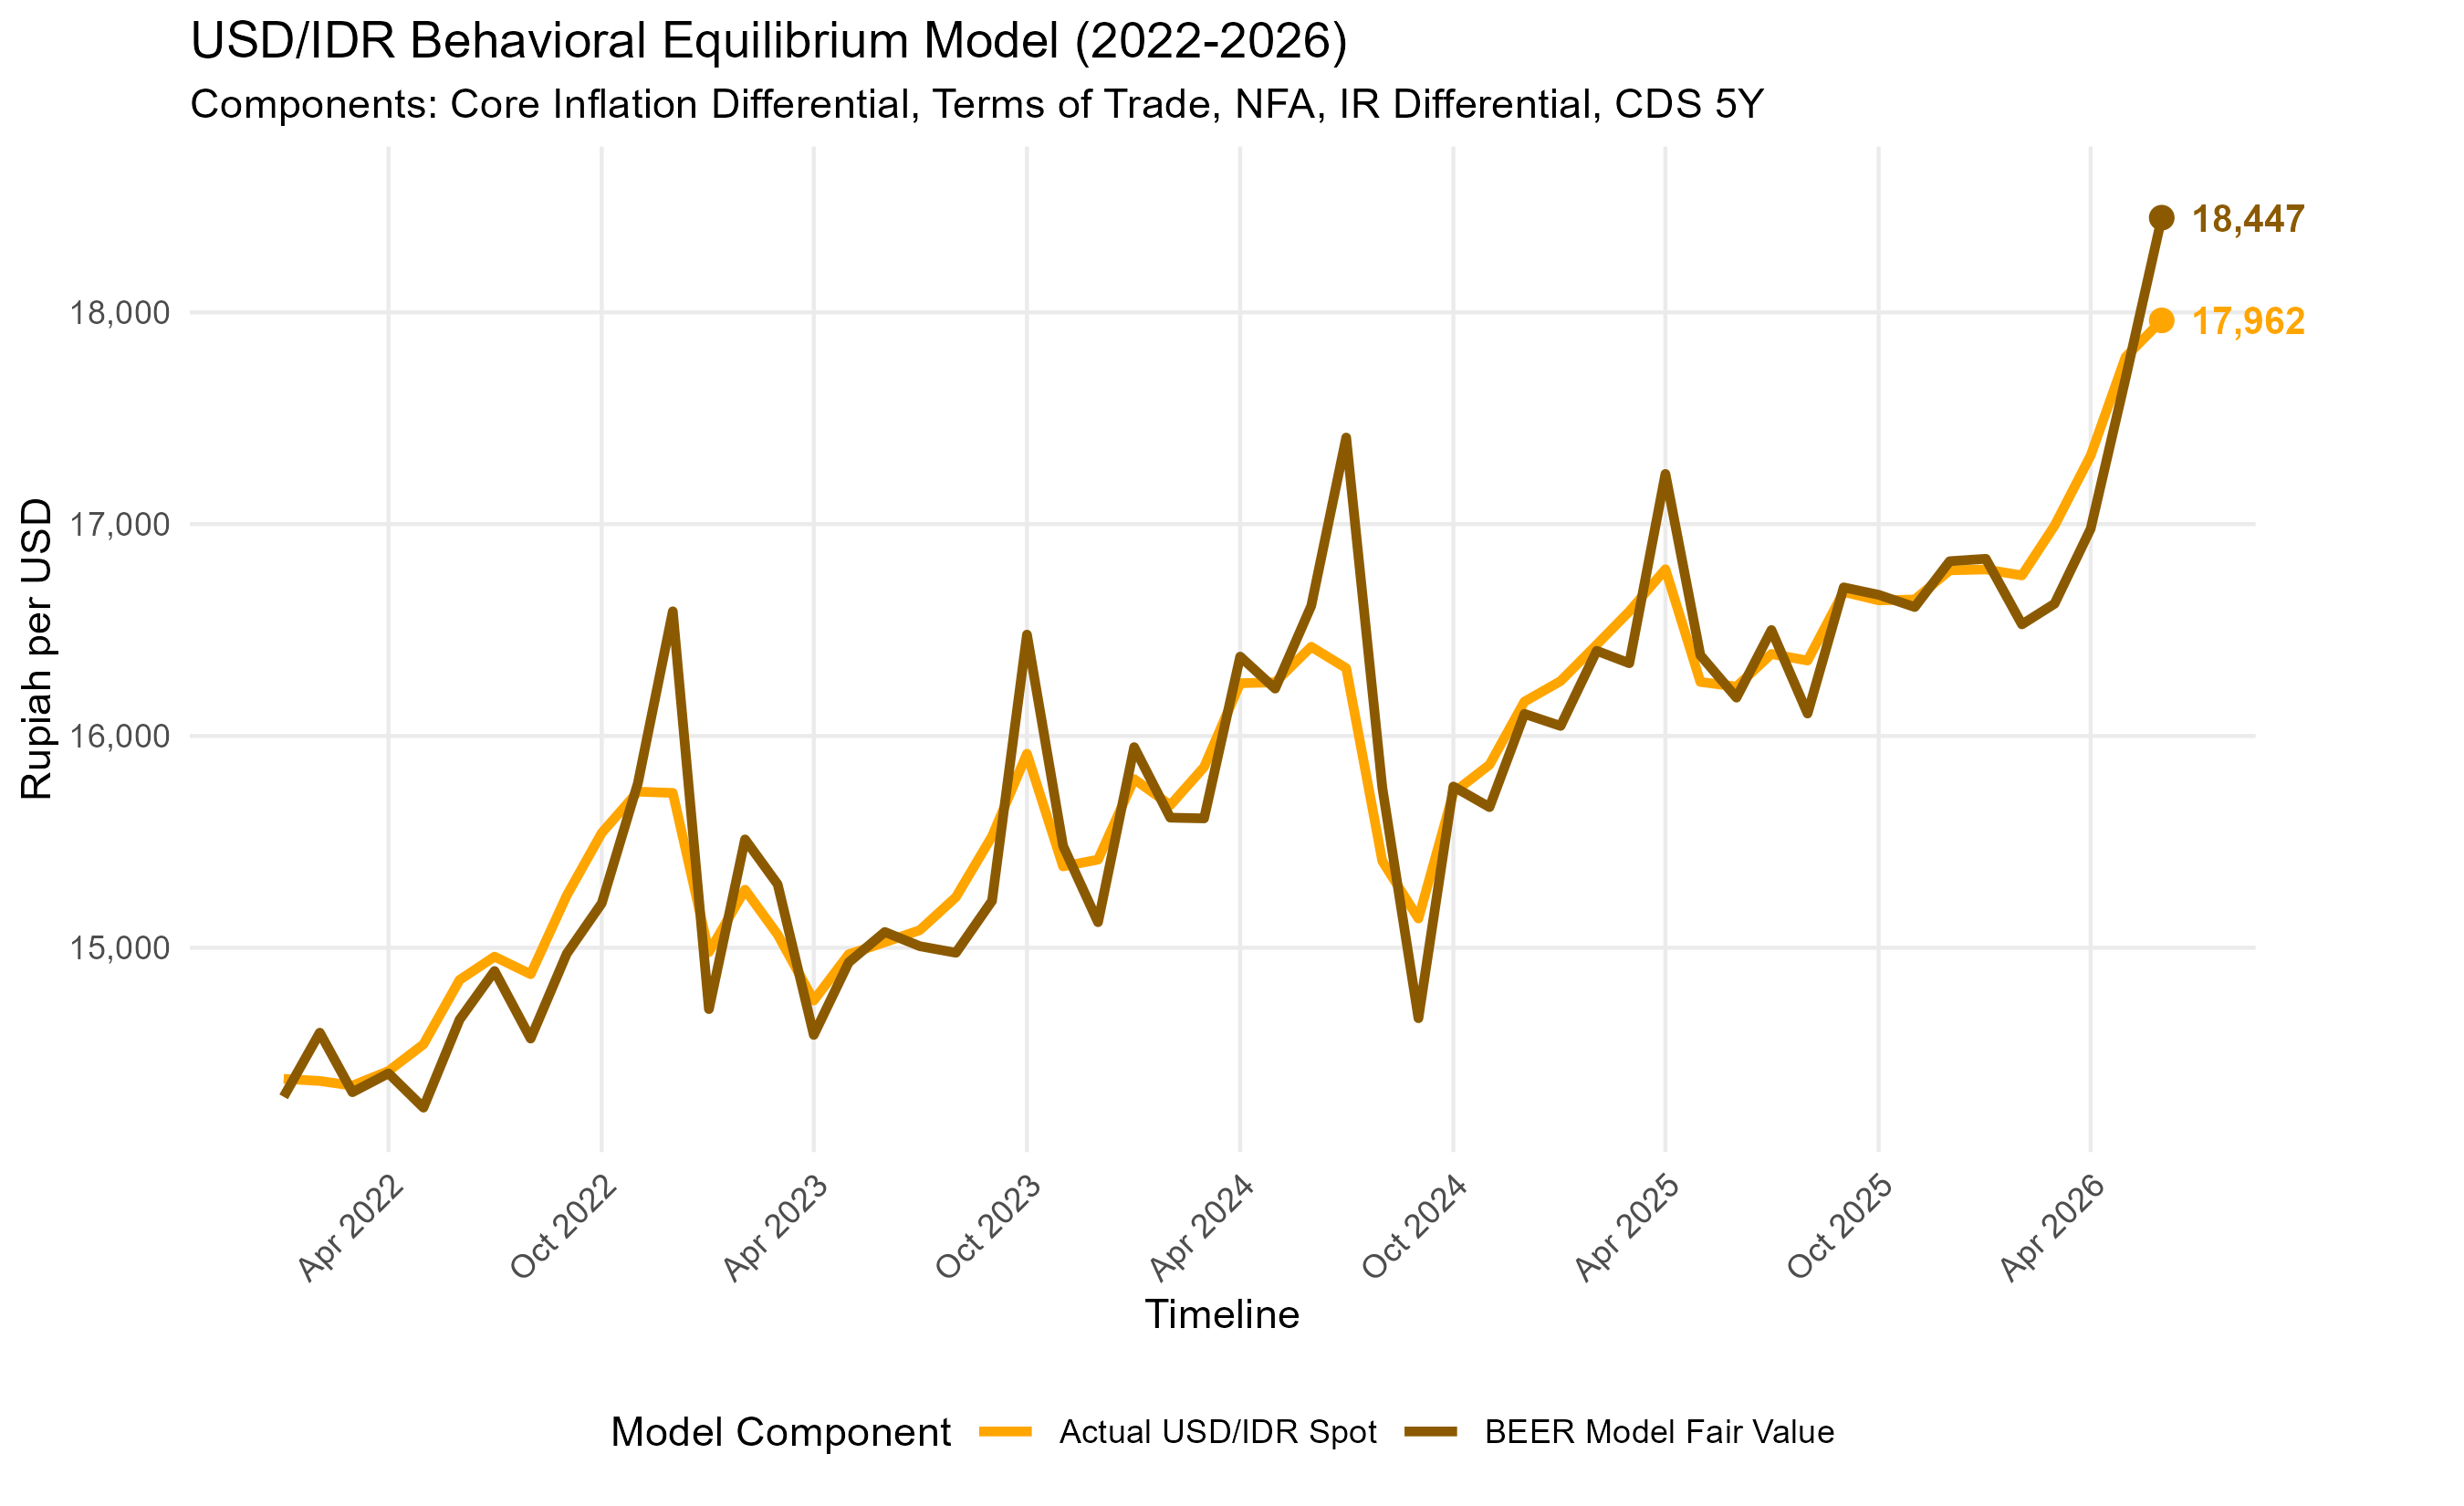
\includegraphics[keepaspectratio]{fig/fair_value_2022_2026.png}}

}

\caption{\label{fig-fair-value}Actual USD/IDR spot rate and BEER model
fair value, January 2022--June 2026. Source: authors' calculations;
underlying data from Bank Indonesia, Bloomberg, World Bank, and IMF.}

\end{figure}%

The fair value tracks the actual rate closely over most of the window,
with the actual rate oscillating around the model-implied equilibrium.
This behavior is consistent with the error-correction interpretation of
the cointegrating relationship. Episodes where the fair value spikes
above the actual rate (late 2022, late 2023, mid-2024, and April 2025)
correspond to periods in which fundamentals and risk pricing
deteriorated faster than the spot rate adjusted. At the end of the
sample (June 2026), the actual rate stands at Rp17,962 per USD against a
fair value of Rp18,447, implying that the Rupiah trades approximately
2.6 percent stronger than the level consistent with current
fundamentals.

The strong caveat must be reserved for the last two most recent
observations (May and June 2026), however. Several fundamentals in
\(Z_t\) like notably the terms of trade and net foreign assets are
published with a lag and is not available yet for May and June 2026 as
the time of writing. The latest available readings are carried forward
for these months. These estimates are therefore subject to revision as
soon as the underlying data become available.

\subsection{Historical Decomposition: Full
Sample}\label{historical-decomposition-full-sample}

Figure~\ref{fig-hd-full} presents the historical decomposition of the
exchange rate based on Equation~\ref{eq-fundamentals} through
Equation~\ref{eq-domestic-sentiment}. The x-axis is the monthly timeline
from March 2010 to June 2026 and the y-axis is the cumulative structural
shock contribution to the log exchange rate, in log deviations from the
deterministic baseline; because \(xr\) is in logarithms, a value of 0.05
corresponds roughly to 5 percent of depreciation pressure. Positive bars
indicate depreciation pressure on the Rupiah and negative bars indicate
appreciation pressure. The bars stack the three shock groups:
fundamentals (orange), external sentiment (dark brown), and domestic
sentiment (red). Source: authors' calculations from the SVAR.

\begin{figure}[htbp!]

\centering{

\pandocbounded{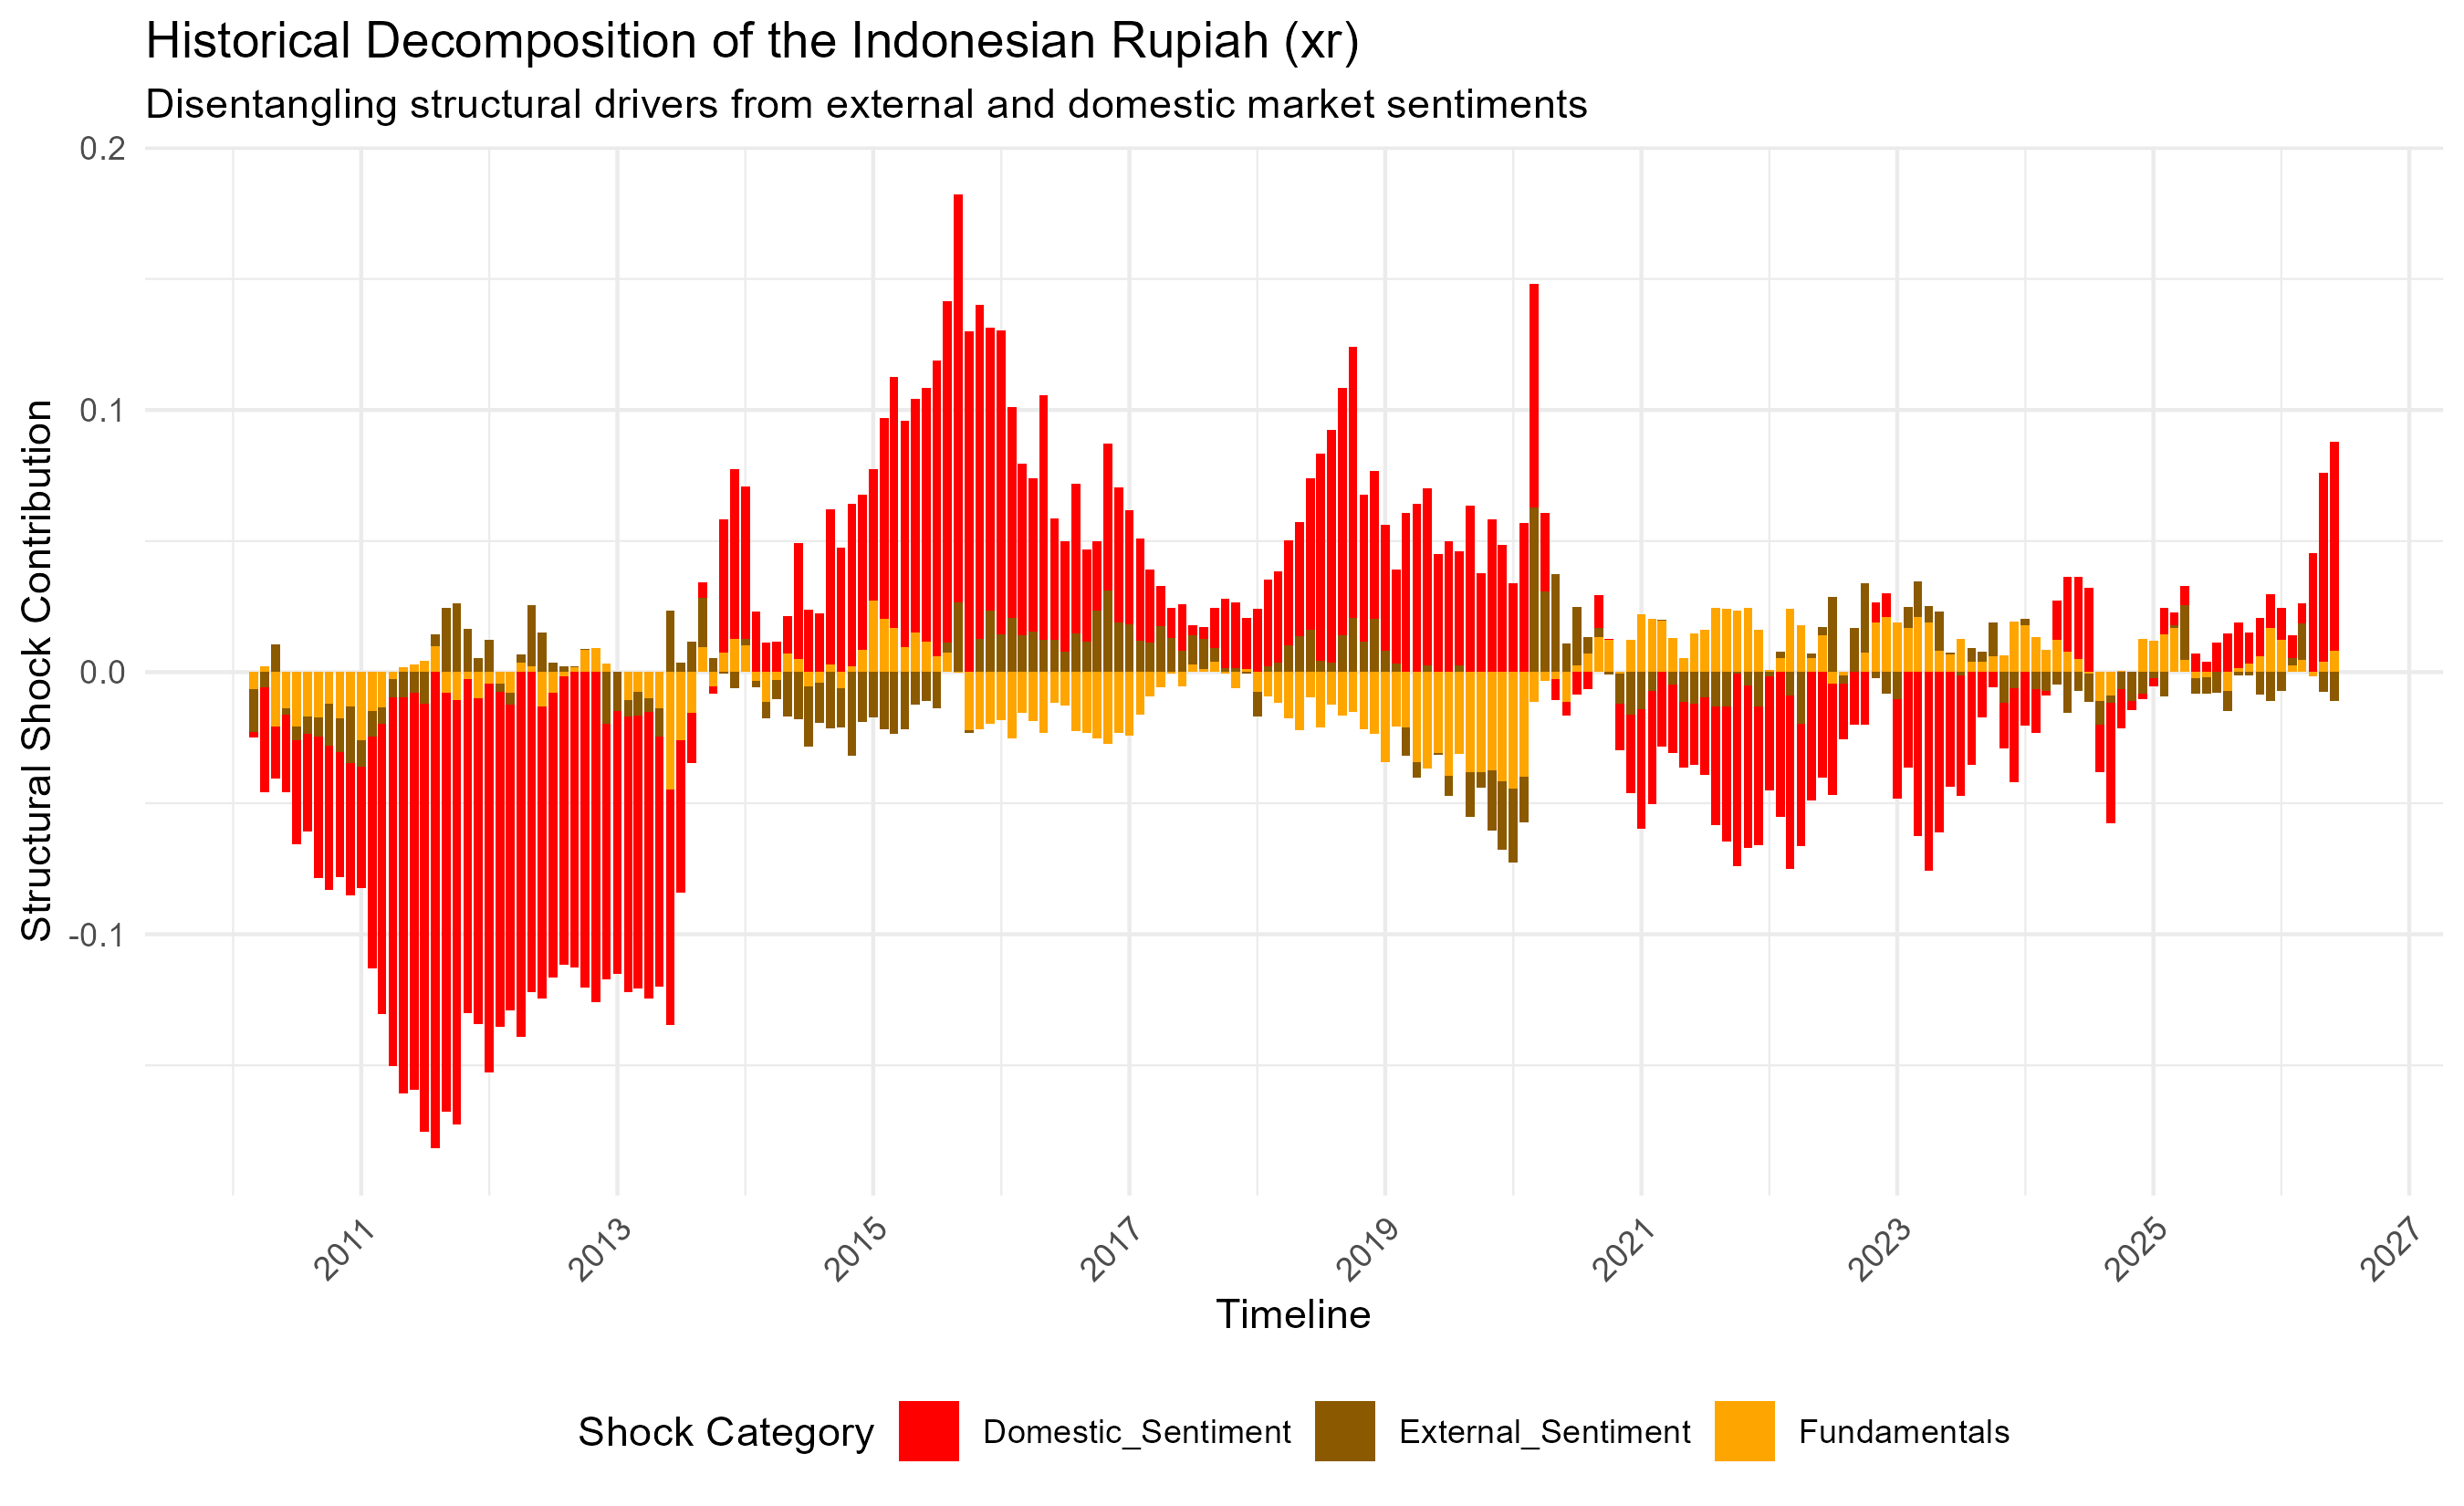
\includegraphics[keepaspectratio]{fig/hd_full_sample.png}}

}

\caption{\label{fig-hd-full}Historical decomposition of the USD/IDR
exchange rate by structural shock group, March 2010--June 2026. Source:
authors' calculations.}

\end{figure}%

Three features stand out. First, domestic sentiment shocks dominate the
amplitude of the decomposition throughout the sample: the large
appreciation pressure of 2011--2013, the depreciation episodes of
2015--2016 and 2018--2019, and the renewed appreciation pressure of
2021--2023 are all predominantly attributable to the domestic sentiment
component. Second, external sentiment contributes episodically rather
than continuously. Its largest imprints coincide with well-identified
global risk events, including the 2013 taper tantrum, the COVID-19 shock
in early 2020, and again in early 2026. Third, fundamentals deliver
comparatively modest but persistent contributions, providing
appreciation support during 2019--2020 and mild depreciation pressure
from 2023 onward. The sample ends with a sharp build-up of depreciation
pressure, again led by domestic sentiment.

\subsection{Historical Decomposition: Recent Twelve
Months}\label{historical-decomposition-recent-twelve-months}

Figure~\ref{fig-hd-12m} zooms the same decomposition into the most
recent twelve months, July 2025 to June 2026. The axes and shock
groupings are identical to Figure~\ref{fig-hd-full}; only the window
differs.

\begin{figure}[htbp!]

\centering{

\pandocbounded{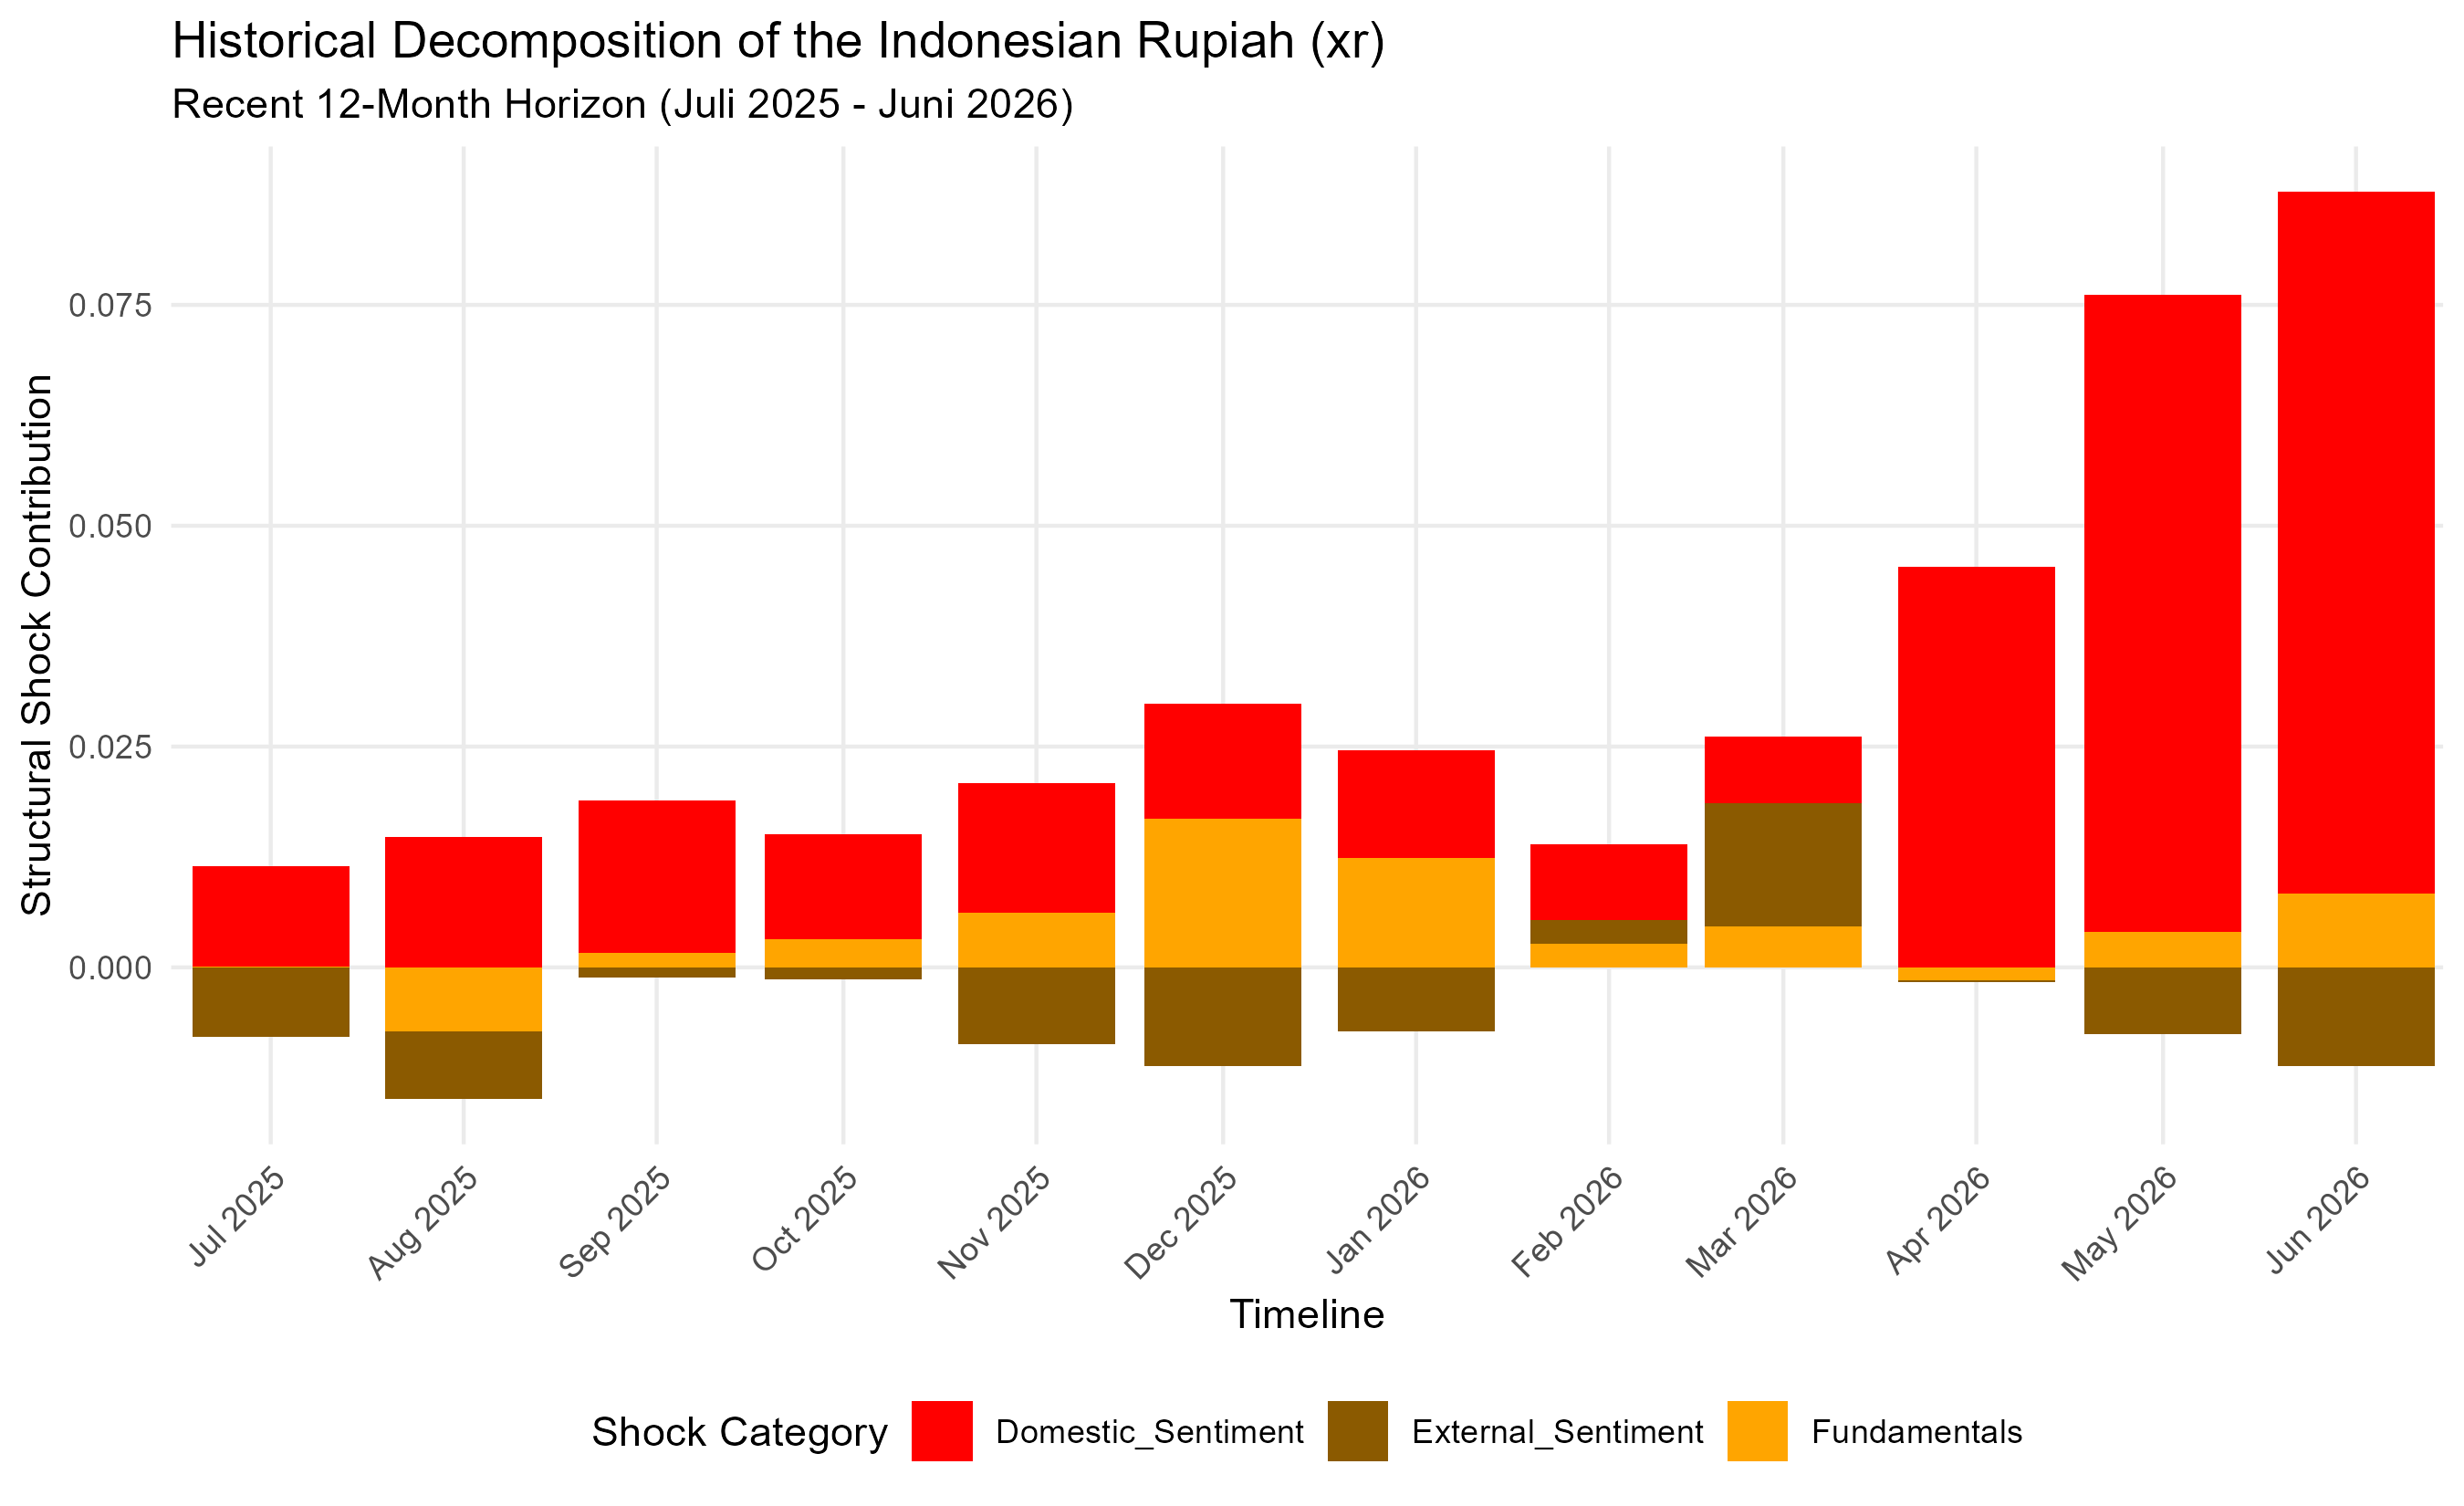
\includegraphics[keepaspectratio]{fig/hd_last_12m.png}}

}

\caption{\label{fig-hd-12m}Historical decomposition of the USD/IDR
exchange rate, July 2025--June 2026. Source: authors' calculations.}

\end{figure}%

Depreciation pressure builds steadily over the window. Through late 2025
the total contribution is modest (below 0.03) and its composition is
mixed: fundamentals account for a sizeable share in December 2025 and
January 2026, while external sentiment is mostly a small offsetting
(appreciation) factor.

The composition shifts markedly in the final quarter. In March 2026,
external sentiment posts its largest positive contribution of the
window, but from April to June 2026 the acceleration is driven almost
entirely by domestic sentiment, whose contribution rises to roughly 0.08
by June 2026 while fundamentals remain small and external sentiment
turns negative.

The recent weakening of the Rupiah therefore reflects domestic
currency-market sentiment rather than a deterioration in fundamentals,
which is the same conclusion suggested by the fair-value gap in
Figure~\ref{fig-fair-value}. As with the fair value, the decomposition
for May and June 2026 rests on fundamentals data that are carried
forward pending release, and both months will be updated once the
underlying data become available.

\section{Interpretation and Policy
Implications}\label{interpretation-and-policy-implications}

\subsection{The BEER Framework for Exchange Rate
Assessment}\label{the-beer-framework-for-exchange-rate-assessment}

The BEER approach provides a systematic way to assess whether a
country's exchange rate is consistent with economic fundamentals (Clark
and MacDonald 1998). The estimated BEER can be interpreted as the level
of the exchange rate that is consistent with the current values of the
economic fundamentals. A departure of the actual exchange rate from the
BEER suggests misalignment, which may be unsustainable in the long run
(Clark and MacDonald 1998).

As noted by Clark and MacDonald (1998):

\begin{quote}
``The methodology of the BEER\ldots{} implies that a departure of the
actual real exchange rate from the estimated BEER will not be
sustainable, as the cointegrating vector of variables operates as an
attractor that eventually brings the actual exchange rate back into line
with the value consistent with the fundamentals.''
\end{quote}

\subsection{Policy Relevance}\label{policy-relevance}

The model has several important policy applications:

\begin{enumerate}
\def\labelenumi{\arabic{enumi}.}
\item
  Exchange Rate Surveillance: The BEER provides a benchmark for
  assessing whether the Rupiah is overvalued or undervalued relative to
  fundamentals, supporting the conduct of exchange rate policy.
\item
  Identification of External Shocks: The historical decomposition
  distinguishes between shocks originating from global commodity prices,
  sovereign risk perceptions, and domestic factors, helping policymakers
  understand the drivers of exchange rate movements.
\item
  Capital Flow Management: The separate identification of external
  sentiment (proxied by the CDS spread) allows policymakers to assess
  the impact of global financial conditions on the Rupiah and design
  appropriate policy responses.
\item
  Monetary Policy Transmission: The interest rate differential variable
  captures the monetary policy transmission mechanism to the exchange
  rate, providing insights into the effectiveness of monetary policy in
  stabilizing the currency.
\end{enumerate}

\subsection{Limitations and Future
Research}\label{limitations-and-future-research}

While the BEER approach offers significant advantages for exchange rate
assessment, several limitations should be acknowledged (Clark and
MacDonald 1998):

\begin{enumerate}
\def\labelenumi{\arabic{enumi}.}
\item
  Model Specification: The BEER approach does not directly incorporate
  considerations of internal and external balance, which are central to
  the FEER approach. Future research could calibrate the fundamentals at
  values corresponding to full employment and sustainable current
  account positions.
\item
  Identification of Fundamentals: The distinction between transitory and
  permanent components of the fundamentals requires judgment, and the
  use of smoothing procedures such as the Hodrick-Prescott filter is
  mechanical and may not correspond to economic notions of sustainable
  levels.
\item
  Emerging Market Specificities: While the model incorporates sovereign
  risk through the CDS spread, other factors specific to emerging
  markets (such as financial dollarization, capital account
  restrictions, and institutional quality) could be incorporated in
  future extensions.
\item
  Forecasting Performance: Future research could evaluate the
  out-of-sample forecasting performance of the model, following the
  approach of MacDonald (1997) and MacDonald and Marsh (1997), who
  demonstrated that BEER-type models have good forecasting properties
  relative to a martingale process.
\end{enumerate}

\section{Appendix: Mathematical Derivations and Code
Implementation}\label{appendix-mathematical-derivations-and-code-implementation}

\subsection{Johansen Cointegration
Framework}\label{johansen-cointegration-framework}

The Johansen procedure for cointegration analysis involves the following
steps:

Step 1: Specify the VAR model of order \(p\):

\[
Y_t = \mu + \sum_{i=1}^{p} A_i Y_{t-i} + u_t
\]

Step 2: Reparameterize into VECM form:

\[
\Delta Y_t = \mu + \Pi Y_{t-1} + \sum_{i=1}^{p-1} \Gamma_i \Delta Y_{t-i} + u_t
\]

Step 3: Compute the likelihood ratio test for the rank of \(\Pi\):

\[
TR = T\sum_{i=r+1}^{N} \ln(1 - \lambda_i)
\]

Step 4: Impose identifying restrictions on \(\beta\) and \(\alpha\)
matrices.

\subsection{SVAR Identification}\label{svar-identification}

The Cholesky decomposition follows these steps:

Step 1: Estimate the reduced-form VAR and obtain \(\Sigma_u\).

Step 2: Compute the Cholesky decomposition:

\[
\Sigma_u = PP'
\]

where \(P\) is lower triangular.

Step 3: Set \(B_0^{-1} = P\) and \(B_0 = P^{-1}\).

Step 4: Compute structural innovations:

\[
\varepsilon_t = B_0 u_t = P^{-1} u_t
\]

\subsection{Historical Decomposition}\label{historical-decomposition-1}

The historical decomposition algorithm proceeds as follows:

Step 1: Compute the moving average coefficient matrices:

\[
\Phi_s = \sum_{i=1}^{p} \Phi_{s-i} A_i, \quad \Phi_0 = I_K
\]

Step 2: Compute structural impulse responses:

\[
\Theta_s = \Phi_s B_0^{-1}
\]

Step 3: For each time \(t\) and shock \(j\):

\[
H_{i,j,t} = \sum_{s=0}^{t-1} \theta_{ij,s} \varepsilon_{j,t-s}
\]

\subsection{Variable Definitions
Summary}\label{variable-definitions-summary}

Table~\ref{tbl-variables} summarizes the definition and data source of
each variable in the endogenous vector \(Y_t\).

\begin{longtable}[]{@{}
  >{\raggedright\arraybackslash}p{(\linewidth - 4\tabcolsep) * \real{0.1628}}
  >{\raggedright\arraybackslash}p{(\linewidth - 4\tabcolsep) * \real{0.4651}}
  >{\raggedright\arraybackslash}p{(\linewidth - 4\tabcolsep) * \real{0.3721}}@{}}
\caption{Variable Definitions and Data
Sources}\label{tbl-variables}\tabularnewline
\toprule\noalign{}
\begin{minipage}[b]{\linewidth}\raggedright
Variable
\end{minipage} & \begin{minipage}[b]{\linewidth}\raggedright
Definition
\end{minipage} & \begin{minipage}[b]{\linewidth}\raggedright
Source
\end{minipage} \\
\midrule\noalign{}
\endfirsthead
\toprule\noalign{}
\begin{minipage}[b]{\linewidth}\raggedright
Variable
\end{minipage} & \begin{minipage}[b]{\linewidth}\raggedright
Definition
\end{minipage} & \begin{minipage}[b]{\linewidth}\raggedright
Source
\end{minipage} \\
\midrule\noalign{}
\endhead
\bottomrule\noalign{}
\endlastfoot
\(xr_t\) & Natural log of USD/IDR nominal exchange rate & Bank
Indonesia, Bloomberg \\
\(infl\_diff_t\) & Core inflation differential (Indonesia - USA) & Bank
Indonesia, BLS \\
\(tot_t\) & Terms of trade (export/import price ratio) & Bank Indonesia,
World Bank, IMF IFS \\
\(nfa_t\) & Net foreign assets / GDP & Bank Indonesia, IMF IIP \\
\(ir\_diff_t\) & Short-term interest rate differential & Bank Indonesia,
U.S. Federal Reserve \\
\(cds_t\) & 5-year sovereign CDS spread & Bloomberg \\
\end{longtable}

\section*{Reproducibility Statement}\label{reproducibility-statement}
\addcontentsline{toc}{section}{Reproducibility Statement}

The model replication package is hosted in the
\href{https://www.github.com/den-econ/beer/}{DEN public GitHub
repository}.

\phantomsection\label{refs}
\begin{CSLReferences}{1}{1}
\bibitem[\citeproctext]{ref-ClarkMacDonald1998}
Clark, Peter B., and Ronald MacDonald. 1998. {``Exchange Rates and
Economic Fundamentals: A Methodological Comparison of BEERs and
FEERs.''} \emph{IMF Working Paper} WP/98/67.

\bibitem[\citeproctext]{ref-Edwards1989}
Edwards, Sebastian. 1989. \emph{Real Exchange Rates, Devaluation, and
Adjustment}. Cambridge, MA: MIT Press.

\bibitem[\citeproctext]{ref-Elbadawi1994}
Elbadawi, Ibrahim. 1994. {``Estimating Long-Run Equilibrium Real
Exchange Rates.''} In \emph{Estimating Equilibrium Exchange Rates},
edited by John Williamson. Washington, DC: Institute for International
Economics.

\bibitem[\citeproctext]{ref-Faruque1995}
Faruque, Hamid. 1995. {``Long-Run Determinants of the Real Exchange
Rate: A Stock-Flow Equilibrium Approach.''} \emph{IMF Staff Papers} 42:
80--107.

\bibitem[\citeproctext]{ref-Johansen1991}
Johansen, Søren. 1991. {``Estimation and Hypothesis Testing of
Cointegration Vectors in Gaussian Vector Autoregressive Models.''}
\emph{Econometrica} 59: 1551--1580.

\bibitem[\citeproctext]{ref-Johansen1995}
Johansen, Søren. 1995. \emph{Likelihood-Based Inference in Cointegrated
Vector Autoregressive Models}. Oxford: Oxford University Press.

\bibitem[\citeproctext]{ref-MacDonald1995}
MacDonald, Ronald. 1995. {``Long-Run Exchange Rate Modeling: A Survey of
the Recent Evidence.''} \emph{IMF Working Paper} WP/95/xx.

\bibitem[\citeproctext]{ref-MacDonald1997a}
MacDonald, Ronald. 1997. {``What Determines Real Exchange Rates? The
Long and Short of It.''} \emph{Journal of International Financial
Markets, Institutions and Money} 7: 207--239.

\bibitem[\citeproctext]{ref-MacDonaldMarsh1997}
MacDonald, Ronald, and Ian Marsh. 1997. {``On the Fundamentals of
Exchange Rates.''} \emph{Journal of International Money and Finance} 16:
765--783.

\bibitem[\citeproctext]{ref-Sims1980}
Sims, Christopher A. 1980. {``Macroeconomics and Reality.''}
\emph{Econometrica} 48: 1--48.

\bibitem[\citeproctext]{ref-Taylor1993}
Taylor, John B. 1993. {``Discretion Versus Policy Rules in Practice.''}
\emph{Carnegie-Rochester Conference Series on Public Policy} 39:
195--214.

\end{CSLReferences}

\end{document}
